% Appendices: material moved out of the main text in the integrator revision (model breadth, ask-policy arithmetic, frontier limits).
\appendix
\section{Model Breadth: The Default Is Not a Prompt Artifact}\label{sec:robust}

\paragraph{Legend test.}
The prompt includes a legend that explains the cue vocabulary, which might itself push models toward assuming that no cue is present. We tested this on bare polarity inputs from \jmlegFamilies{} families (human-written and machine-written; draw~1) with \jmbreadthOrigModels{} models in three arms: (a) the prompt with the legend, (b) the prompt with no legend, and (c) the legend plus the instruction that markers may be missing and neither reading should be assumed. The rule was fixed before generation: the default is an artefact if arm (b) or arm (c) falls below 90\% affirmative. Among committed outputs, the affirmative share was \jmlegendAff{}\% [\jmlegendAffLo{}, \jmlegendAffHi{}] with the legend, \jmlegendNoLegendAff{}\% [\jmlegendNoLegendAffLo{}, \jmlegendNoLegendAffHi{}] with no legend and \jmlegC{}\% [\jmlegCLo{}, \jmlegCHi{}] with the explicit instruction (\jmlegAN{}, \jmlegBN{} and \jmlegCN{} outputs). Removing the legend moves the share by \jmlegBminusA{} points [\jmlegBminusALo{}, \jmlegBminusAHi{}] and the explicit instruction by \jmlegCminusA{} [\jmlegCminusALo{}, \jmlegCminusAHi{}]. The instruction does not make models abstain: the commitment rate is \jmlegACommit{}\% with the legend and \jmlegCCommit{}\% with the instruction. A second independent draw gives \jmlegDrawTwoA{}\%, \jmlegDrawTwoB{}\% and \jmlegDrawTwoC{}\%, and the lowest single model--arm cell is \jmlegMinModelNoLegend{}\% (an API model with no legend). The pre-declared verdict is that the default is not a legend artefact.

\paragraph{Model breadth.}
We repeated the bare, no-legend and cue arms on two further open models, one from a fourth family, so that the study covers \jmbreadthModels{} models from \jmbreadthFamilies{} families (the \jmbreadthOrigModels{} original models plus Qwen2.5-14B and Mistral-Nemo-12B; open models are 4-bit quantised GGUF builds, and none is frontier scale). Table~\ref{tab:breadth} gives the per-model cells. Every model chooses the affirmative reading on at least \jmbreadthMinAff{}\% of bare polarity inputs; the lowest legend-test arm is \jmbmMinLegendArm{}\%; the cue gain on polarity is at least \jmbreadthPolChipMin{} points for every model; and the speech-act cue contrast ranges from \jmbreadthSpeechChipMin{} to \jmbreadthSpeechChipMax{} points, with a lower writer-cluster bound above zero for every model. Across the \jmbmCells{} model-by-dimension cells, the cue beats an irrelevant cue with a lower bound above zero in \jmbmIrrelCells{}, and a plain word matches the cue within 5 points in \jmbmWordEqCells{}. With the full sentence as input, critical-commitment match stays at or above \jmbmFullMin{}\% in every model and dimension, so the failures belong to the compressed input and not to the generators' ability to follow a commitment.

\begin{table}[t]
\caption{Model breadth (human-written pairs, writer-cluster bootstrap for gains; legend test draw~1). Affirmative share on bare polarity inputs and with no legend; cue gain on polarity (cue minus a non-critical word, points); speech-act cue contrast (points); plain word minus cue on speech act (points; positive means the word did better).}\label{tab:breadth}
\small
\begin{tabular}{lccccc}
\toprule
Model & Bare aff.\ (\%) & No legend (\%) & Polarity gain & Speech-act gain & Word $-$ cue (act) \\
\midrule
Qwen2.5-7B & \jmbmQwenSBare{} & \jmbmQwenSNoLeg{} & \jmbmQwenSPolGain{} & \jmbmQwenSActGain{} & \jmbmQwenSActWord{} \\
Llama-3.1-8B & \jmbmLlamaBare{} & \jmbmLlamaNoLeg{} & \jmbmLlamaPolGain{} & \jmbmLlamaActGain{} & \jmbmLlamaActWord{} \\
Gemma-3-4B & \jmbmGemmaBare{} & \jmbmGemmaNoLeg{} & \jmbmGemmaPolGain{} & \jmbmGemmaActGain{} & \jmbmGemmaActWord{} \\
GPT-6.1-terra (API) & \jmbmTerraBare{} & \jmbmTerraNoLeg{} & \jmbmTerraPolGain{} & \jmbmTerraActGain{} & \jmbmTerraActWord{} \\
Qwen2.5-14B & \jmbmQwenLBare{} & \jmbmQwenLNoLeg{} & \jmbmQwenLPolGain{} & \jmbmQwenLActGain{} & \jmbmQwenLActWord{} \\
Mistral-Nemo-12B & \jmbmNemoBare{} & \jmbmNemoNoLeg{} & \jmbmNemoPolGain{} & \jmbmNemoActGain{} & \jmbmNemoActWord{} \\
\bottomrule
\end{tabular}
\end{table}

\paragraph{A further family.}
A Gemini Flash-Lite model, run through its public API under a daily quota, gives \jmgemA{}\% (legend) and \jmgemC{}\% (explicit instruction) affirmative on the same \jmgemN{} families with a commitment rate of \jmgemCommit{}\%, so the legend result holds in a further family. The cue arms for this model are incomplete under the quota and are not analysed; the model is an additional machine replication of the default and is not part of the \jmbreadthModels{}-model estimates.

\paragraph{Bound.}
One prompt template per arm, one wording of the legend instruction, quantised open models and a single API model per proprietary family. The result says that the default does not depend on the legend; it does not say that no prompt could change it.

% ------------------------------------------------------------------------------------------------

\section{Ask-Policy Arithmetic: No Policy Beats Random}\label{sec:asks}

If a cue costs a tap, a system could spend taps only where a cue is likely to be missing. We tested ranking rules for a budget of \jmaskBudgetPct{}\% of messages on the \jmtTwoUnits{} elicitation units: a no-model-call keyword prior, model confidence from a forced-choice probe, an entropy stand-in, shortest keywords first, and a generic few-shot clarification trigger in the style of CLAM, all against a gated random baseline (random among messages whose keywords lack the cue). The arithmetic assumes that the user supplies the cue when asked. At the \jmaskBudgetPct{}\% budget the polarity reversals per 1,000 were \jmdpAlwaysCommitPol{} [\jmdpAlwaysCommitPolLo{}, \jmdpAlwaysCommitPolHi{}] with no asks, \jmdpAskPriorPol{} [\jmdpAskPriorPolLo{}, \jmdpAskPriorPolHi{}] for the keyword prior, \jmdpAskRandPol{} [\jmdpAskRandPolLo{}, \jmdpAskRandPolHi{}] for gated random and \jmclamPol{} [\jmclamPolLo{}, \jmclamPolHi{}] for the CLAM-style trigger. None of the \jmaskPrimaryN{} named contrasts survives correction (\jmaskPrimarySig{} significant); prior minus gated random on polarity is $\jmaskPriorMinusRandPol$ per 1,000 [$\jmaskPriorMinusRandPolLo$, $\jmaskPriorMinusRandPolHi$], and the CLAM-style trigger minus gated random is $\jmclamDiffPol$ [$\jmclamDiffPolLo$, $\jmclamDiffPolHi$] (Holm $p=\jmclamPHolmPol{}$); on politeness it is $\jmclamDiffPolite$ [$\jmclamDiffPoliteLo$, $\jmclamDiffPoliteHi$]. The minimum detectable effect is \jmaskMdePol{} per 1,000 for the prior contrast (\jmaskMdeRelPol{}\% of the always-commit rate) and \jmclamMdePol{} for the CLAM-style contrast, so this is a null of limited power, not an equivalence. Within the cost accounting of this section, the efficient move is to elicit the cue, and the open problem is how a writer supplies it, not which message to ask about.

% ------------------------------------------------------------------------------------------------

\begin{figure}[t]
\centering
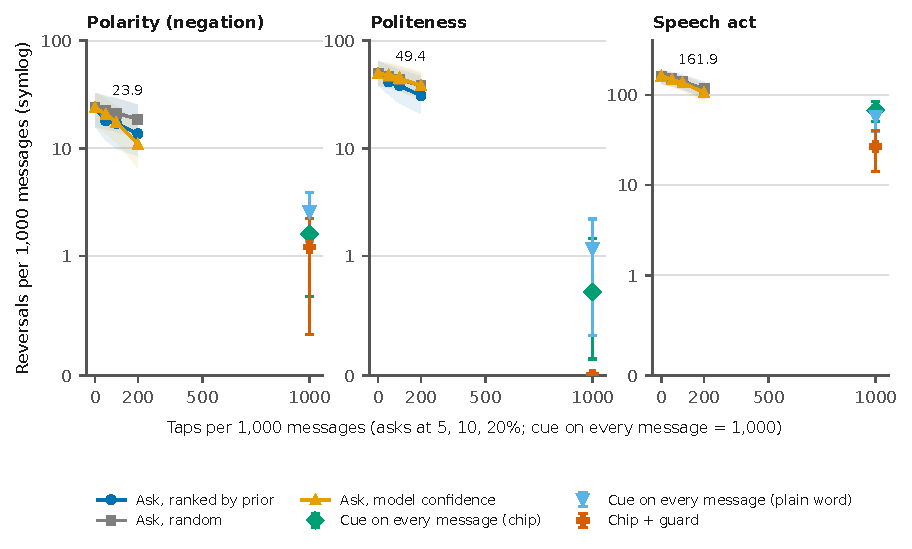
\includegraphics[width=\linewidth]{figs/fig3_frontier.pdf}
\caption{Reversals per 1,000 messages against taps per 1,000 messages, by dimension. Lines: ask policies at 5, 10 and 20\% of messages (ranking arithmetic; assumes an asked writer supplies the cue). Points: cue on every message, measured on stored outputs (chip, plain word, chip plus guard), with 95\% intervals. Ask policies are not distinguishable from gated-random at matched taps; polarity is \jmdpAskPriorPol{} (prior-ranked) vs \jmdpAskRandPol{} (random) at 10\% taps. Vertical axis is symlog.}\label{fig:frontier}
\Description{Reversals per 1,000 messages against taps per 1,000 messages, by dimension.}
\end{figure}


\section{Frontier Limits: Asking, Model Uncertainty and Partner Context}\label{sec:frontier}

The preceding results suggest several tempting ways to avoid supplying a cue on every message: ask the writer only when it matters, let the model's own uncertainty decide, or let the conversation partner's last remark supply context.
We tested each in a controlled, machine-labelled study.
All labels in this subsection are machine labels (two judges with a blind arbiter), the studies are pilot-scale and post-pilot rounds are marked as such in the evidence files, and no human has yet checked them.

\paragraph{Ask policies.}
The ask-policy comparison of Section~\ref{sec:asks} (Figure~\ref{fig:frontier}) is the first of these tests: no ranking rule, including a clarification-style trigger, beats asking at random among messages that lack the cue at matched taps, and supplying the cue on every message (\jmfOneRevPolChip{} polarity reversals per 1,000 with a chip, \jmfOneRevPolWord{} with a plain word) undercuts them.
A learned gate that uses model internals averts a modest share of SLP-weighted speech-act reversals under simulated resolution rates, but a supervised entropy-feature learner matches it; we treat that study as an evaluation framework and not as a result.

\paragraph{The model's own uncertainty does not flag the reversals.}
We asked whether default decoding hides a calibrated distribution over the dropped negation, using \jmknsModels{} local models, an untruncated sampler and \jmknsUnitsCap{} messages in which the negation was removed from every keyword string (a stress test) and a set of human keyword messages. % CITE-NEEDED: semantic entropy; contextual calibration
For Qwen2.5-7B, the model for which both datasets agree, sampled negation appears in \jmknsCapSampled{}\% of samples against a source rate of \jmknsCapTarget{}\% on the stress set, and in \jmknsHumSampled{}\% against \jmknsHumTarget{}\% on human keywords: the model is overconfident, not hiding a calibrated tail.
The sampled share ranks which inputs lost their negation at AUROC \jmknsAucKOneSixQwen{} and \jmknsAucKOneSixLlama{} for the two models, against \jmknsAucLex{} for a model-free classifier on the keywords alone.
A continuous score from the negation-token probability mass reaches \jmknsAucNegmass{} (\jmknsAucNegmassLo{} to \jmknsAucNegmassHi{}); its difference from the keyword classifier is $\jmknsNegmassVsLex$ [$\jmknsNegmassVsLexLo$, $\jmknsNegmassVsLexHi$], so a per-input signal exists but is no better than a model-free one.
A verbalised-probability score from one API model reaches \jmknsAucTerraVerbal{}, a difference of $\jmknsTerraVsLex$ [$\jmknsTerraVsLexLo$, $\jmknsTerraVsLexHi$] from the keyword classifier; its interval touches zero, so we treat it as a lead for a confirmatory run and not as a result.
The conclusion for design is that the model cannot be asked whether it dropped a cue more cheaply than the writer can be asked for the cue.

\paragraph{Partner context improves defaults and adds an echo.}
Giving the model the conversation partner's last remark is a published way to improve expansion accuracy~\cite{cai2022abbrev}, and we tested whether it also moves the polarity default.
With \jmpcFamilies{} polarity families, \jmpcModels{} models and model-written partner remarks, a negative remark raises the share of negated bare output by $\jmpcAll$ points [$\jmpcAllLo$, $\jmpcAllHi$], mostly by echoing the remark or agreeing with it.
Excluding verbatim echoes and agreement replies, the excess is $\jmpcProp$ points [$\jmpcPropLo$, $\jmpcPropHi$]; it depends on who wrote the remarks, from $\jmpcAuthQwen$ with one remark author to $\jmpcAuthMistral$ with the other on the \jmpcAuthFamilies{} families written by both.
A supplied polarity cue largely removes it: the excess is $\jmpcCue$ points [$\jmpcCueLo$, $\jmpcCueHi$] when echoes and agreements are counted as harm, and $\jmpcCueLow$ [$\jmpcCueLowLo$, $\jmpcCueLowHi$] when they are not.
A question remark does not raise the affirmative default; it lowers the affirmative share by $\jmpcQAff$ points through abstention.
The study is a controlled demonstration with templated remarks.
It says nothing about the rate in real AAC conversation or about whether echoing a remark the writer agrees with is harmful, and no zero-tap mitigation we tried beat random asking at matched taps.

\paragraph{What the limits establish.}
Taken together, these results fix the role of the cue.
Asking, model uncertainty and partner context each reduce reversals only partly or at a tap cost that a cue-on-every-message policy undercuts on the measured dimensions, and the cue still has to be elicited from the writer.
The remaining problem is not the trigger but covering the writer's whole intended message from a compressed input, which Sections~\ref{sec:waterfall} and~\ref{sec:req-revisions} show is a question about approval-gated drafts and not about a better filter.
